\section{Kompasy w grach (Zofia Sosińska)}\label{chap:skrm}
\footnotetext{Internet, \url{https://www.youtube.com/watch?v=AIZUd9brK3c}, dostęp: 06.09.2023}
Częstą funkcjonalnością gier jest możliwość eksploracji świata, w którym na gracza czekają przygody i zadania do wykonania.
Jednak przestrzeń przygotowana dla użytkownika może być na tyle duża i skomplikowana, że powstaje ryzyko 
zgubienia się. Jednym ze sposobów jakim projektanci gier wyciągają rękę do użytkownika jest danie mu
kompasu. Może to być bardzo proste narzędzie, pokazujące jedynie strony świata, immitujące klasyczny przedmiot ze świata rzeczywistego.
Już taka garstka informacji potrafi uprościć graczowi odnalezienie drogi do celu. Jednak innym podejściem jest rozszerzenie
funkcjonalności kompasu o pokazywanie pozycji innych ważnych punktów odniesienia, celów, do których trzeba się dostać lub 
kluczowych postaci.

\textit{The Elder Scrolls V: Skyrim} (skrótowo \textit{Skyrim})\footnote{\url{https://elderscrolls.bethesda.net/en}} jest to fabularna gra
wyprodukowana przez Bethesda Game Studios i wydana przez Bethesda Softworks. Autorzy przygotowali dla gracza duży świat,
który ten może dowolnie eksplorować. Nawigację oparli o bardzo pomocne i sprytne rozwiązanie,
jakim jest pasek przedstawiający pole widzenia gracza. Służy on między innymi jako kompas, ponieważ 
jedną z jego mechanik jest pokazanie użytkownikowi stron świata, znajdujących się w kierunku, w którym 
on patrzy. Pasek ułatwia także poruszanie się po świecie, sygnalizując położenie wrogów, kompanów i ważnych 
dla rozgrywki lokalizacji.

\begin{figure}[htbp]
	\centering
	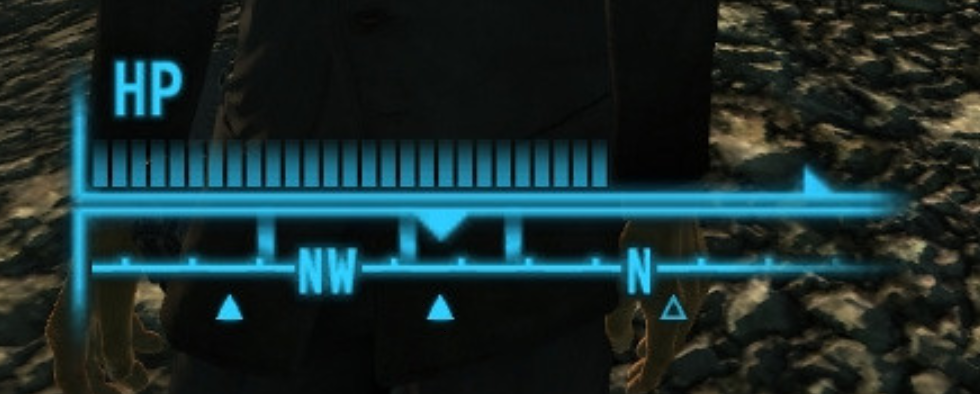
\includegraphics[width=0.9\textwidth]{images/ui/compassSkyrim.png}
	\caption[Kompas z gry \textit{Skyrim}.]{Kompas z gry \textit{Skyrim}\protect\footnotemark.}\label{fig:Fallout}
\end{figure}
\footnotetext{Internet, \url{https://www.youtube.com/watch?v=nr62-GnrrOs}, dostęp: 05.09.2023}
